\documentclass{article}
\usepackage{graphicx} % Required for inserting images
\setlength{\parskip}{1em}

\title{Point light importance sampling}
\author{Roman Vasilyev}
\date{June 2025}

\begin{document}

\maketitle

\section{Uniform sampling}
Let's say we have a scene with many point lights. Computing the incoming illumination from all the lights might be too computationally heavy.
So instead, we sample one light at a time. If each light is equally likely to be chosen, the process is called \textbf{uniform sampling}.

Let's simplify the scene to 3 point lights with their power in absolute values being 2, 5 and 20.
Say we want to calculate the incoming radiance at some point on a surface.
For simplicity, let the incoming irradiance from those point lights be attenuated to 1, 2, and 15 respectively when the light reaches the shading point. So, the total would be 18.

\begin{figure}[h]
    \centering
    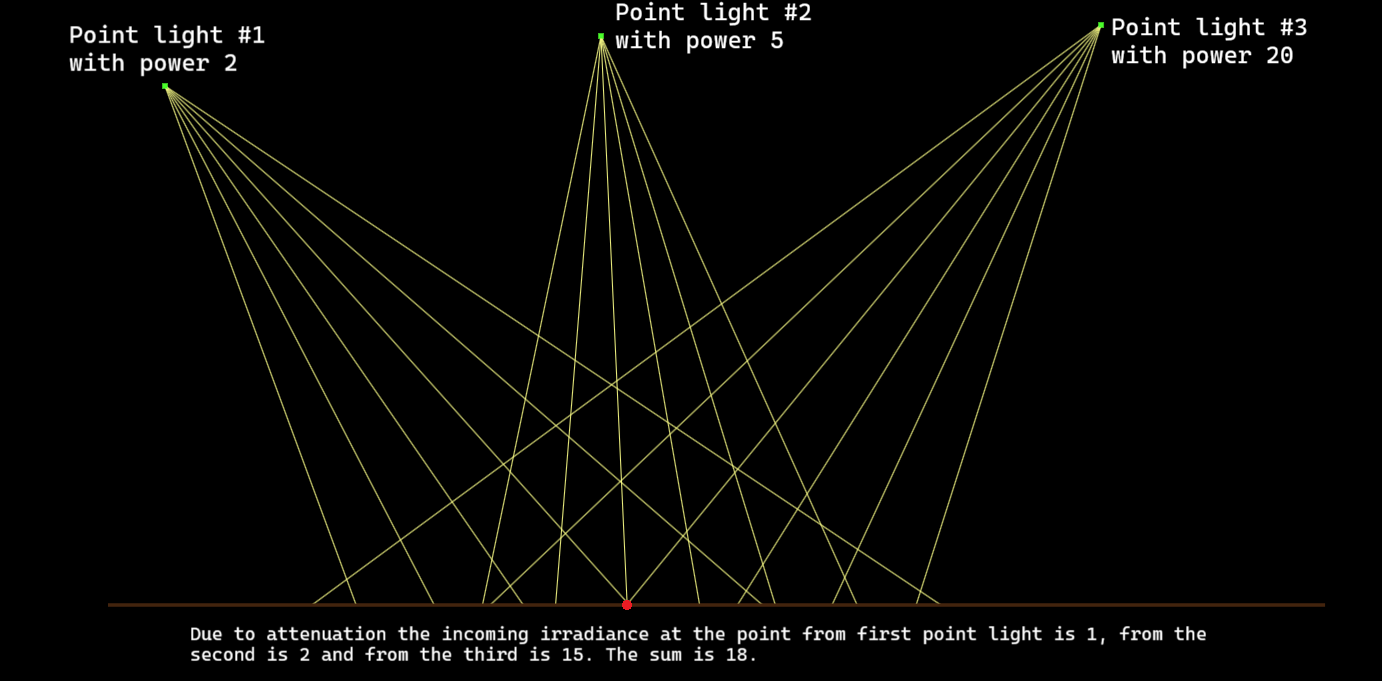
\includegraphics[width=\textwidth]{a.png}
    \caption{Initial setup}
    \label{fig:enter-label}
\end{figure}

Here's the general formula for computing average on N sampled values:

\[Average = \frac{1}{n} \displaystyle\sum_{i=0}^{n} \frac{s_i}{pdf_i}\]

We take uniformly 3 samples, divide each sampled value by the \textbf{pdf} of the sample (\textbf{pdf} = 1/3, because it's uniform) and then
average it by dividing their sum by 3 (because we took 3 samples).\
The result would be 18:

\[Li = \frac{\frac{1}{\frac{1}{3}} + \frac{2}{\frac{1}{3}} + \frac{15}{\frac{1}{3}}}{3} = \frac{3 + 6 + 45}{3} = 18\]

But what if some point lights are way stronger than the others? We want to sample them more often. And, to help us here, comes...
\section{Importance sampling}

To do so we will use the same formula, but we need a way to sample the point light №3 ten times more often that the light №1. Because it's ten times more powerful.
But the only \textbf{rng} we have on the GPU can generate a random float within [0, 1] interval.

An \textbf{alias table} here comes to our aid. It's a table where each entry has a threshold and alias. For our case the table would look like this:

\begin{center}
  \begin{tabular}{ | l | c | c | c | }
    \hline
    &Light №1 & Light №2 & Light №3 \\ \hline
    Threshold & $\frac{2 * 3}{27}$ & $\frac{5 * 3}{27}$ & 1 \\ \hline
    Alias & 2 & 2 & 2 \\
    \hline
  \end{tabular}
\end{center}

The algorithm for generating that table can be found in D. Knuth's ``The art of Computer Programming''.

How to work with this table?
It works as follows:
\begin{itemize}
    \item Generate a uniform random float \textbf{U\textsubscript{1}} in range \textbf{[0, 1]} and multiply it by the number of lights to get \textbf{N} - light index.
    \item Generate a uniform random float \textbf{U\textsubscript{2}} in range \textbf{[0, 1]} and compare it with the \textbf{Threshold} value of light \textbf{N}.
    \item If \textbf{U\textsubscript{2}} is smaller than the \textbf{Threshold}, and \textbf{N} remains the same.
    \item If \textbf{U\textsubscript{2}} is greater that the \textbf{Threshold}, then the \textbf{N} is replaced with the value from the alias table.
\end{itemize}

Let's check how it works. The initial chance of selecting Light №1 is $\frac{1}{3}$. Then $\frac{6}{27}$ is the chance that \textbf{U\textsubscript{2}} would be smaller than \textbf{Threshold} and \textbf{N} would remain the same.
\begin{itemize}
    \item $\frac{1}{3} * \frac{6}{27} = \frac{2}{27} $ - chances of picking the 1st point light.
    \item $\frac{1}{3} * \frac{15}{27} = \frac{5}{27} $ - chances of picking the 2nd point light.
\end{itemize}

What are the chances of picking the 3rd light.
They are the sum of the chances of picking it: instead of 1st point light, instead of the second light and  $\frac{1}{3}$, which comes from the cases when original \textbf{U\textsubscript{1}} selects it.

$\frac{1}{3} * (1 - \frac{6}{27}) + \frac{1}{3} * (1 - \frac{15}{27}) + \frac{1}{3} = $

$\frac{1}{3} * \frac{21}{27} + \frac{1}{3} * \frac{12}{27} + \frac{1}{3} = $

$\frac{7}{27} + \frac{4}{27} + \frac{9}{27} = $

$\frac{20}{27}$

As you can see, the sum of probabilities adds to one:

$\frac{2}{27} + \frac{5}{27} + \frac{20}{27} = 1$

And the chances of sampling the 3rd light are 10 times higher than those of the 1st light:

$\frac{\frac{20}{27}}{\frac{2}{27}} = 10$

Now we have a way to non-uniformly sample our point light.
Now, let's verify that if we sample the light this way the final result would stay the same.
With this new sampling method we can say that on average, if we take 27 samples, 2 of them would be of the first light, 5 of the second and 20 of the third.

$Li = \frac{2 * \frac{1}{\frac{2}{27}} + 5 \frac{2}{\frac{5}{27}} + 20 * \frac{15}{\frac{20}{27}}}{27} =$

$\frac{27 + 27 * 2 + 27 * 20}{27} = $

$ = 18$

Yep, we got the same result. Although it appears we used more samples to compute the average result (27 instead of 3),
in practice more important (that's why it's called importance sampling) values would come first
and the result would converge way faster.

\end{document}
